\documentclass[a4paper,12pt]{article}
\usepackage[utf8]{inputenc}
\usepackage[IL2]{fontenc}
\usepackage{listings}
\usepackage{amssymb}
\usepackage{amsmath}
\usepackage{url}
\usepackage{graphicx}
\usepackage[czech]{babel}
\usepackage[top=2cm, bottom=2cm, left=2cm, right=2cm]{geometry}
\usepackage{paralist}
\usepackage{url}
\begin{document}
\thispagestyle{empty}
\vfill
\begin{center}
{\Large \bf Masarykova univerzita\\[1ex]}
{\large Přírodovědecká fakulta}
\end{center}
\vfill
\begin{center}

\includegraphics[scale=0.7]{prf_logo.pdf}
\end{center}
\begin{center}
\vfill

Marek Bryša, Jan Kovář\\[3em]
{\LARGE \bf Kolektivní investování}\\[1em]
SEMINÁRNÍ PRÁCE\\
\vfill

{2012}
\end{center}

\setcounter{page}{0}
\newpage

\tableofcontents
\newpage

\section*{Úvod}
\addcontentsline{toc}{section}{Úvod}

V~této práci popíšeme fondy kolektivního investování jako jednu z~alternativ, jak nakládat s~dočasně volnými peněžními prostředky. Nejprve se zaměříme na výhody a nevýhody těchto fondů, které popíšeme v~následující části. Poté popíšeme jednotlivé typy fondů kolektivního investování, tedy investiční fondy a podílové fondy, a vysvětlíme, jakou roli hrají v~kolektivním investování investiční společnosti. Na závěr se zaměříme na možnosti investování do fondů kolektivního investování v~České republice.

\section{Výhody a nevýhody kolektivního investování}

Kolektivní investování je definováno v zákoně č. 189/2004 Sb., o kolektivním investování (\cite{zakon}).

Kolektivní investování je podnikání, jehož předmětem je
shromažďování peněžních prostředků upisováním akcií investičního fondu nebo vydáváním
podílových listů podílového fondu, investování na principu rozložení rizika a další
obhospodařování tohoto majetku.

My se však na kolektivní investování podíváme z~pohledu investora. Kolektivní investování jako jedna z~možností nakládání s~volnými peněžními prostředky přináší řadu výhod a nevýhod, které popíšeme v~této kapitole. 

\medskip

\noindent Mezi výhody kolektivního investování patří:
\begin{compactitem}
\item \emph{Diverzifikace rizika} - prostřednictvím fondů kolektivního investování můžeme investovat do velkého množství na sobě nezávislých titulů, a to i~s~relativně malým objemem investovaných prostředků. 

\item \emph{Snížení transakčních nákladů} - díky kolektivnímu investování můžeme realizací jedné investice investovat do mnoha instrumentů současně a dosáhnout tak úspory na poplatcích a dalších transakčních nákladech. Navíc obchodování instrumentů ve velkých objemech může přinést úspory z~rozsahu.
\item \emph{Likvidita vložených prostředků} - likvidita podílových listů otevřených podílových fondů je zajištěna právem podílníka na zpětný odkup. Likvidita uzavřených fondů je zajištěna obchodováním na sekundárním trhu.
\item \emph{Profesionální správa majetku} - fond spravují profesionální odborníci, kteří sledují dění na kapitálových trzích. Investor tedy nemusí mít hluboké znalosti o~finančních trzích a jejich instrumentech. 
\item \emph{Možnost investovat do titulů, ke kterým by se drobný investor samostatně nedostal} - některé investice (např. státní dluhopisy, nemovitosti) mohou být podmíněny relativně vysokou hodnotou investice, na kterou by většina investorů sama nedosáhla. Prostřednictvím fondů kolektivního investování se však na takových investicích mohou podílet i drobní investoři.
\item \emph{Dohled regulátorů} - fondy kolektivního investování podléhají regulaci České národní banky.
\end{compactitem}

\medskip

\noindent
Na druhou stranu,  kolektivního investování přináší také některé nevýhody:
\begin{compactitem}
\item \emph{Správní poplatky} - investor zpravidla platí roční poplatky za správu svěřeného majetku. Poplatky jsou také většinou spojeny s nákupem či prodejem podílových listů nebo akcií.
\item \emph{Omezení investiční volnosti} - investor se vzdává práva rozhodovat o~konkrétních titulech, které chce mít ve svém portfoliu. Může pouze ovlivnit oblast, do které chce investovat, a to prostřednictvím volby typu fondu. 
\item \emph{Konflikt zájmu mezi investory a správci portfolia} - investor a správce portfolia mohou mít odlišné zájmy ohledně podstoupeného rizika, či očekávané výnosnosti.
\item \emph{Často podprůměrná výkonnost fondů} - výkonnost fondu by měla být porovnávána s~určitým měřítkem, tzv. benchmarkem.
\item \emph{Riziko investování} - jedná se o~standardní rizika spojená se vstupem na kapitálové trhy, zejména riziko poklesu hodnoty investice v~případě nepříznivého vývoje finančních trhů.
\end{compactitem}

\section{Subjekty kolektivního investování}
Mezi fondy kolektivního investování patří investiční fondy a podílové fondy. V~této kapitole popíšeme, jaký je mezi nimi rozdíl a jakou roli hrají v~kolektivním investování investiční společnosti.
 
\subsection{Investiční společnost}
Investiční společnost je právnická osobu, jejímž předmětem podnikání je kolektivní investování. Investiční společnost může
\begin{compactitem}
\item zakládat podílové fondy a spravovat majetek do nich vložený,
\item obhospodařovávat majetek investičních fondů na základě smlouvy o~obhospodařování.
\end{compactitem}
Ke své činnosti musí investiční společnost získat povolení České národní banky.

\subsection{Investiční fond}
Investiční fond je právnická osoba (akciová společnost), jejímž předmětem podnikání je kolektivní investování a která má povolení ČNB k~činnosti investičního fondu. Zakládá se na dobu určitou, maximálně na 10~let. Obchodní firma investičního fondu musí obsahovat označení \emph{uzavřený investiční fond}. Na základě smlouvy o~obhospodařování majetku může investiční fond svěřit obhospodařování svého majetku investiční společnosti. Investiční fond může vydávat pouze akcie stejné jmenovité hodnoty.

\subsection{Podílový fond}
Na rozdíl od investičního fondu nemá podílový fond právní subjektivitu, ale je zakládán investiční společností na základě povolení České národní banky. Investiční společnost shromažďuje prostředky do podílového fondu vydáváním podílových listů. Podílový list je cenný papír, který představuje podíl na majetku podílového fondu. Podílový fond je tedy souborem majetku, který náleží všem vlastníkům podílových listů, tzv. podílníkům, a to dle poměru držených podílových listů.  

\begin{figure}[htb]
\centering
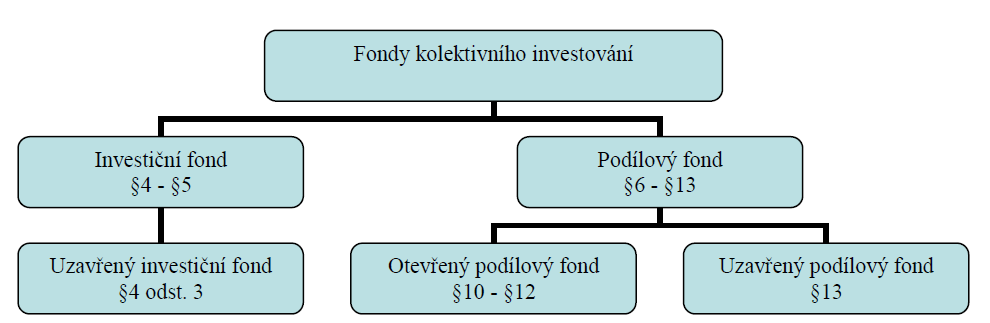
\includegraphics[width=\textwidth]{deleni.png}
\caption{Členění fondů kolektivního investování dle zákona č. 189/2004 Sb., o kolektivním investování, zdroj: \cite{dp}}
\end{figure}

Podle práva na zpětný odkup podílových listů dělíme podílové fondy na otevřené a uzavřené.

\emph{Otevřený podílový fond} má povinnost zpětného odkupu podílových listů za aktuální hodnotu na základě žádosti podílníka, a to nejpozději do 15 pracovních dní od podání žádosti. Otevřený fond nemá předem omezen počet emitovaných podílových listů, nemá tedy omezen počet podílníků.

\emph{Uzavřený podílový fond} má již při svém vzniku stanoven počet podílových listů, které může emitovat. Je zakládán na dobu určitou, po této době vstupuje do likvidace, anebo se změní na otevřený fond.

\section{Vybrané fondy v České republice}
	V této části se seznámíme s konkrétními možnostmi investic do podílových fondů v České republice. Budou uvedeny příklady fondů peněžního trhu, dluhopisového, akciového a investiční program pro zajištění na stáří.
	\subsection{AXA investiční společnost, a.s.}
		Francouzská skupina AXA je druhým největším správcem fondů v Evropě.\cite{axa_about} Její produkty mají v České republice nulové vstupní poplatky, ale klient hradí správní poplatky a výstupní v případě ukončení investice za kratší dobu než 5 let. Kompletní přehled poplatků je uveden v příloze \ref{axa}.
		
		Pro drobné investory jsou určeny všechny fondy se vstupní investicí 5~000 Kč. Výjimkou je AXA Corporate Fund, který má minimální vstupní investici 1~000~000 Kč a následnou 500~000 Kč.
		
		\subsubsection{AXA CZK Konto}
			AXA CZK Konto je otevřený podílový fond, který byl do 31.12.2011 klasifikován jako fond peněžního trhu, od 1.1.2012 se podle metodiky AKAT ČR jedná o smíšený fond.
			\begin{quote}
				Cílem investiční strategie je poskytnout podílníkům růst hodnoty jejich investice za podmínky, že celkový rizikový profil fondu minimalizuje možnost ztráty v horizontu 6 měsíců. Cíle je dosahováno investicemi do široce diverzifikovaného portfolia cenných papírů s fixním nebo variabilním úrokovým výnosem a aktivním řízením úrokového rizika.\footnote{\url{http://www.axa.cz/lide/podilove-fondy/czk-konto/popis}}
			\end{quote}
			
			Doporučeným investičním horizontem je minimálně 6 měsícu. Fond je vhodný pro investora s nízkou tolerancí k riziku, který neočekává vysoký výnos.
			
			Graf zhodnocení fondu je uveden v obrázku \ref{axa_czk_konto}. Fond připsal za 5 let 10.07\%, v průměru tedy 1.93\% ročně, přičemž za poslední rok 0.8\%. To je výrazně méně než nabízely a nabízejí spořící účty v bankách. Je vidět, že v době finanční krize mezi roky 2008 a 2009 byl fond velmi volatilní. 
			\begin{figure}[h!]
		  	\centering
				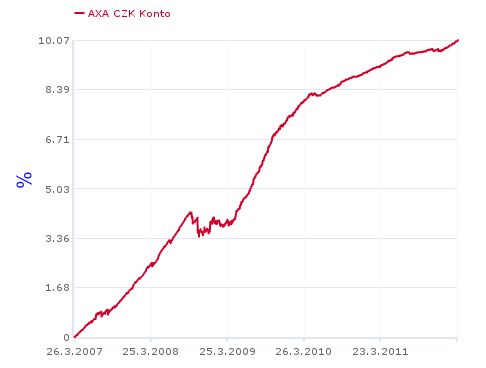
\includegraphics[width=0.6\textwidth]{axa_czk_konto.png}			
				\caption{Graf zhodnocení AXA CZK Konto za 5 let zdroj: http://www.axa.cz/fondy/porovnani/podilove.aspx?fund=29}
				\label{axa_czk_konto}
			\end{figure}
		\subsubsection{AXA CEE Dluhopisový fond}
			AXA CEE Dluhopisový fond je otevřený podílový fond klasifikovaný jako dluhopisový. 
			\begin{quote}
				\footnote{\url{http://www.axa.cz/lide/podilove-fondy/cee-dluhopisovy/popis}}Fond investuje do dluhopisů emitentů všech kategorií:
				\begin{compactitem}
			    \item dluhopisů nadnárodních institucí
			    \item státních dluhopisů
			    \item bankovních dluhopisů
			    \item dluhopisů obchodních společností
			    \item komunálních dluhopisů emitovaných v krajinách střední a východní Evropy			
    	  \end{compactitem}
		  \end{quote}						
			
			Doporučeným investičním horizontem jsou minimálně 3 roky. Fond je určen pro střednědobé investice s mírou rizika i výnosem o něco výššími než u fondu peněžního trhu.
			
			Graf zhodnocení fondu je uveden v obrázku \ref{axa_cee_dluh}. Výnos fondu je za 5 let 10.73\%, což je 2.05\% ročně. To je o málo více než fond CZK Konto, ale s mnohem vyšší volatilitou.
			
			\begin{figure}[h!]
		  	\centering
				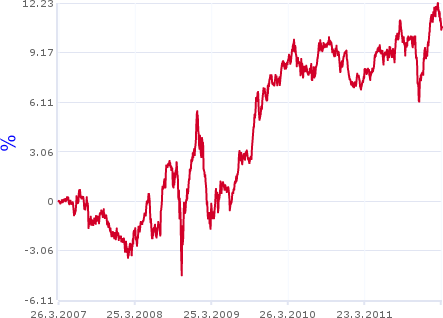
\includegraphics[width=0.6\textwidth]{axa_cee_dluh.png}			
				\caption{Graf zhodnocení AXA CEE Dluhopisový fond za 5 let zdroj: http://www.axa.cz/fondy/porovnani/podilove.aspx?fund=32}
				\label{axa_cee_dluh}
			\end{figure}
		\subsubsection{AXA CEE Akciový fond}
			AXA CEE Akciový fond je oficiálně klasifikován jako akciový fond.
			\begin{quote}
				Cílem fondu je dosahovat co nejvyššího dlouhodobého zhodnocení investic. Majetek fondu je tvořený především akciemi společností, které jsou lídry ve svém odvětví v regionu střední a východní Evropy. Největší podíl na portfoliu mají české, polské a maďarské společnosti. Odvětvová struktura portfolia není omezená, významně se na ní ale podílí energetický, telekomunikační a finanční sektor. Investice jsou směřované také do odvětví farmacie či strojírenství.\footnote{\url{http://www.axa.cz/lide/podilove-fondy/cee-akciovy/popis}}
			\end{quote}
			
			Doporučeným investičním horizontem je minimálně 5 let. Fond pro ivestora slibuje vyskoké zhodnocení v dlouhém obdobi, ale za cenu vysoké střednědobé volatility.
			
			Na grafu \ref{axa_cee_akc} dobře vidíme nebezpečí investic do akciových produktů ve středním období. Za 5 let fond ztratil 27.11\% hodnoty, v době finanční krize dokonce 52.3\%.			
			
			\begin{figure}[h!]
		  	\centering
				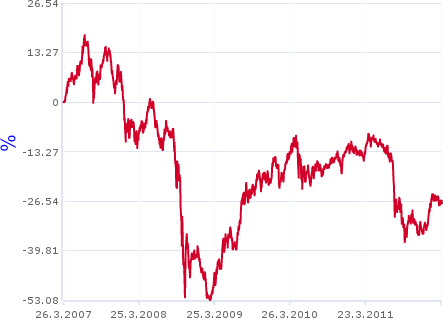
\includegraphics[width=0.6\textwidth]{axa_cee_akc.png}			
				\caption{Graf zhodnocení AXA CEE Akciový fond za 5 let zdroj: http://www.axa.cz/fondy/porovnani/podilove.aspx?fund=28}
				\label{axa_cee_akc}
			\end{figure}
	\subsection{Pioneer Asset Management, a.s. -- Rentier Invest}
		Společnost Pioneer působí na českém trhu od roku 1995. Přímo nabízí investice do fondů v CZK a přes svou lucemburskou matku také rodinu fondů v zahraničních měnách.\cite{pio_about} Pro osobní finance je zajímavým produktem program Rentier Invest.
		
		Program tvoří 7 na sebe navazujících linií s postupně se snižující rizikovostí a výnosem. První linie je určena pro 40-25 let před předpokládaným ukončením investice, druhá pro 25-15 let atd. Podrobný přehled je uveden na obrázku \ref{ri_linie}.
		
		Minimálně je možno investovat poprvé 30 000 Kč, následně 10 000 Kč nebo pravidelně 1 000 Kč. Vstupní polatky se s každou linií snižují, viz obrázek \ref{ri_cost}. Správcovské poplatky nejsou pro tento program na internetu k nalezení.
		
		Na obrázku \ref{ri_graf} je graf výkonnosti Rentier Invets v liniích 1 a 7 v případě jednorázové a pravidelné investice od 6.5.2005 do 23.3.2012. Linie 1 dosáhla za posledních 5 let ztráty 22.08\%, linie 7 zisku 9.27\%. Zde názorně vidíme výhodu pravidelného investování v tom, že se celková hodnota investice rychle navrací i při silném poklesu trhů. Při rychlém nárůstu by to samozřejmě platilo také. Pravidelné investování tedy může působit jako jistý stabilizátor rizika.
		\begin{figure}[h!]
		  	\centering
			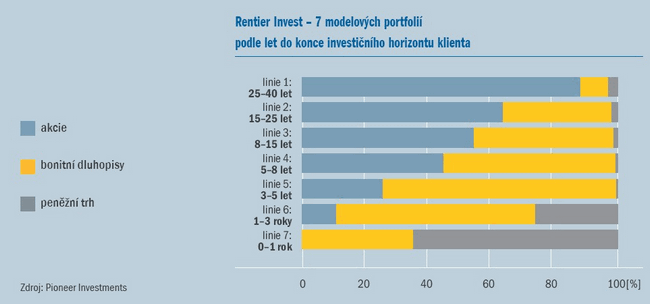
\includegraphics[width=0.8\textwidth]{graf_alokace_linii.png}			
			\caption{Graf alokace linií Rentier Invest zdroj: http://www.pioneerinvestments.cz/ Rentier/ZakladniInformace.asp}
			\label{ri_linie}
		\end{figure}
		\begin{figure}[h!]
		  	\centering
			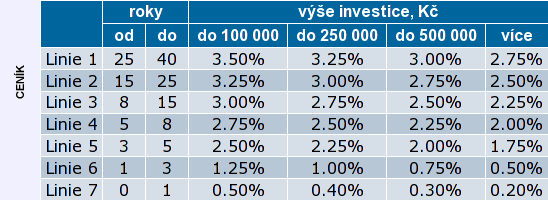
\includegraphics[width=0.6\textwidth]{ri_cost.png}			
			\caption{Poplatky Rentier Invest zdroj: http://www.pioneerinvestments.cz/ Rentier/ZakladniInformace.asp}
			\label{ri_cost}
		\end{figure}
		\begin{figure}[h!]
		  	\centering
			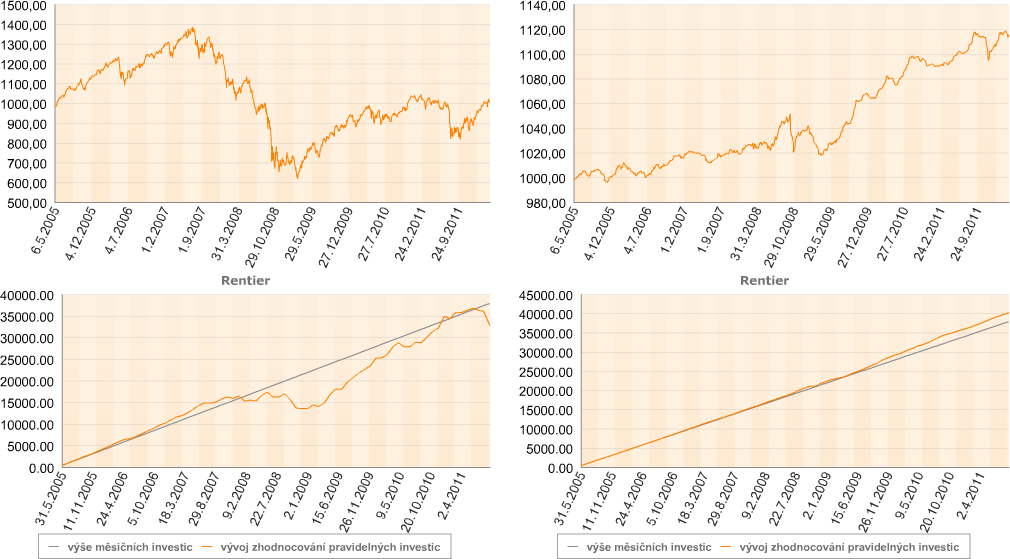
\includegraphics[width=1.0\textwidth]{ri_graf.png}			
			\caption{Výkonnost Rentier Invets v liniích 1 a 7 v případě jednorázové a pravidelné investice od 6.5.2005 do 23.3.2012 zdroj: http://www.pioneerinvestments.cz/Rentier/AktualniInfo.asp?line=1}
			\label{ri_graf}
		\end{figure}
\clearpage
	\section{Závěr}
		V České republice se drobnému střadateli nabízí široká škála produktů kolektivního investování. Existují podílové fondy fondy s nízkým rizikem a tomu odpovídající nízkou výkonností až po silně rizikové, ale potenciálně velmi výkonné. Dále jsou zajímavé investiční programy pro zajištění na stáří, které s přibližujícím se věkem automaticky přesouvají prostředky do méně rizikových instrumentů. Investovat lze do většiny fondů jednorázově i pravidelně, což může vést k nižší střednědobé volatilitě hodnoty investice.
		
		Obecně je kolektivní investování vhodné pro investora, který je nadprůměrně finančne gramotný,  dobře si uvědomuje rizika poklesu hodnoty investice, hledá možnost vyššího zhodnocení ve středním a dlouhém období a chce snadný nástroj k dosažení tohoto cíle. Také je to užitečný způsob diverzifikace úspor.
\clearpage
\appendix
\section{Poplatky AXA investiční společnost}
\label{axa}	
Zdroj:  \cite{axa_cite}\\
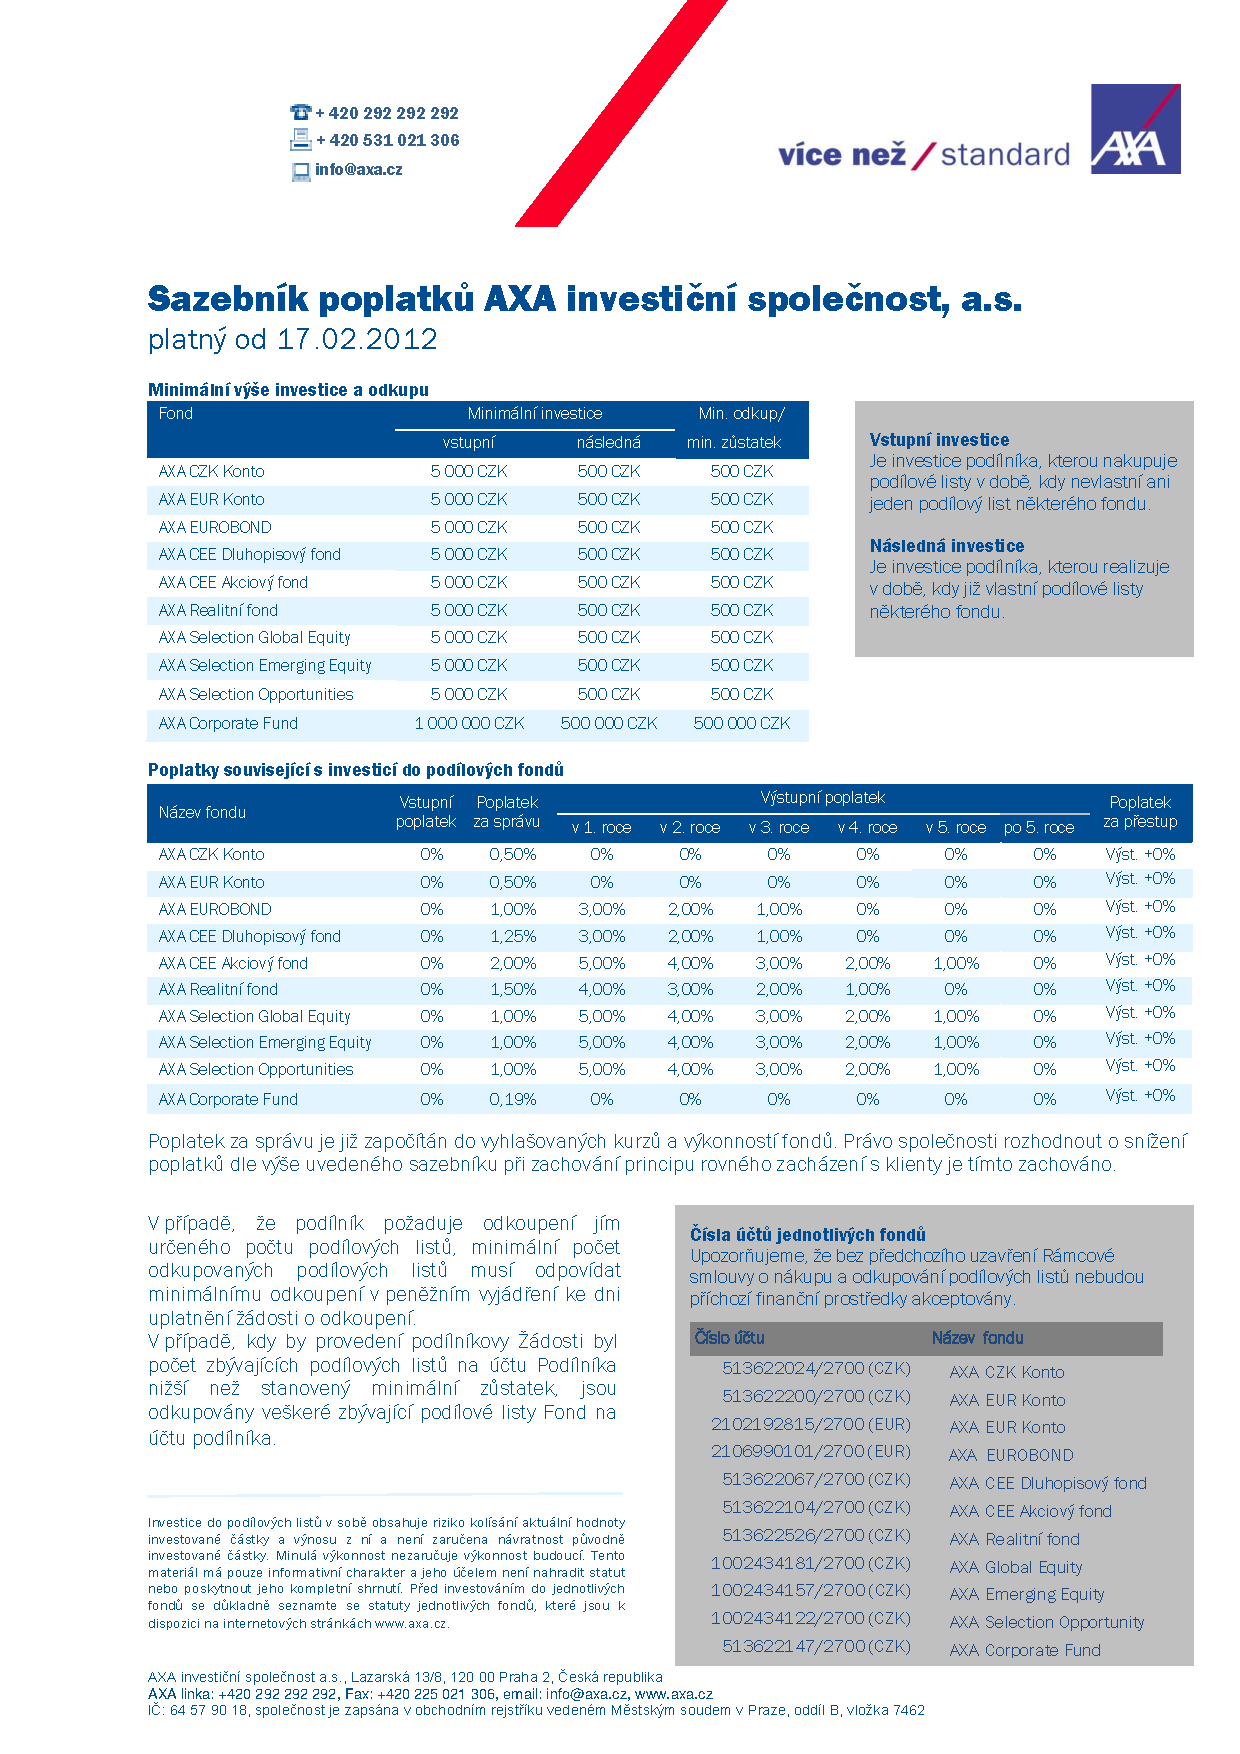
\includegraphics[width=1.0\textwidth]{axa.pdf}
\renewcommand{\bibname}{Seznam použité literatury}
\begin{thebibliography}{9}
\addcontentsline{toc}{section}{Seznam použité literatury}
\thispagestyle{plain}
\bibitem{zakon} Zákon č. 189/2004 Sb., o kolektivním investování
\bibitem{zafi} SVOBODA, Martin. \emph{Základy financí.} 1. vyd. Brno: Masarykova univerzita, 2009, 195 s. ISBN 978-802-1049-765. 
\bibitem{dp} VAŠKOVÁ, Lucie. \emph{Kolektivní investování v České republice.} Brno, 2011. Dostupné z: \url{http://is.muni.cz/th/206629/esf_m/}. Diplomová práce. Masarykova univerzita, Ekonomicko-správní fakulta. Vedoucí práce Ing. Dalibor Pánek.

\bibitem{axa_about}
Leták Podílové fondy AXA, [cit. 2012-03-23], Dostupné z WWW:  \url{http://www.axa.cz/getattachment/59ed8936-2745-409d-952b-801213d54a2d/Letak-Podilove-fondy}


\bibitem{axa_cite}
Sazebník poplatků AXA investiční společnost, a.s., [cit. 2012-03-23], Dostupné z WWW:  \url{http://www.axa.cz/getattachment/edb1852e-a78d-4c80-9515-55f0f1db5953/Sazebnik-poplatku}

\bibitem{pio_about}
Pioneer Asset Management, a.s., O společnosti Pioneer Investments [cit. 2012-03-23], Dostupné z WWW:  \url{http://www.pioneerinvestments.cz/Spolecnost.asp}
\end{thebibliography}
\end{document}